\chapter{Regularization}
In our learning objectice, we had a term correspond to the zero/one loss on the training data, plus a \textbf{regularizer} whose goal was to ensure that the learned function did not overfit. If you replace to zero/one loss with a surrogate loss, you obtain the following objective:
\begin{equation}
    \min_{w,b} \sum_n l(y_n, \vec{w} \cdot \vec{x}_n + b) + \lambda R(\vec{w},b)
\end{equation}
From the discussion of surrogate loss function, we would like to ensure that \(R\) is convex. Otherwise, we will be back to the point where optimization becomes difficult. Beyond that, a common desire is that the components of the weight vector should be small. This is a form of \textbf{inductive bias}.

\section{Regularizers}

If \(w_i\) is reasonably small, this is unlikely to have much of an effect on the classification decision. On the other hand, if \(w_i\) is large, this could have a large effect. 
Another way to say the same thing is to look at the derivative of the predictions as a function of \(w_i\). The derivative of \(\vec{w} \cdot \vec{x} + b\) with respect to \(w_i\) is:
\begin{equation}
    \frac {\delta [\vec{w} \cdot \vec{x} + b]} {\delta w_i} = \frac {\delta [\sum_d w_d x_d + b]} {\delta w_i} = x_i
\end{equation}
Interpreting the derivative as the rate of change, we can see that the range of change of the prediction function is proportional to the individual weights. So if you want the function to change slowly, you want to ensure that the weights stay small.

One way to accomplish this is to simply use the norm of the weight vector. Namely \(R^\text{(norm)}(\vec{w},b) = ||\vec{w}|| = \sqrt{\sum_d w_d^2}\). This function is convex and smooth, which makes it easy to minimize.

An alternative to using the sum of squared weights is to use the sum of absolute weights: \(R^\text{(abs)}(\vec{w},b) = \sum_d |w_d|\).

\section{\(p\)-norm}
The line of thinking leads to the general concept of \(p\)-norms. This is a family of norms that all have the same general flavor. We write \(||\vec{w}||_p\) to denote the \(p\)-norm of \(\vec{w}\).
\begin{equation}
    ||\vec{w}||_p = R(\vec{w},b) = \left[ {\sum_{w_j} |w_j|^p} \right]^{\frac 1 p}
\end{equation}
You can check that the 2-norm exactly corresponds to the usual Euclidean norm, and the 1-norm corresponds to the absolut regularizer described above.

\begin{wrapfigure}{r}{0.35\textwidth}
\begin{center}
    \vspace*{-20pt}
    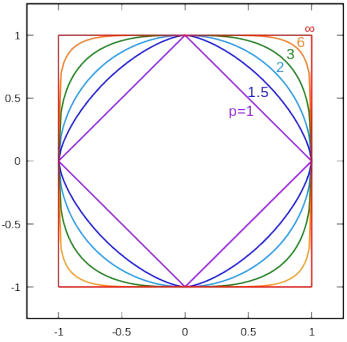
\includegraphics[width=0.35\textwidth]{040}
    \caption{\(p\)-norms visualized}
    \vspace*{-40pt}
\end{center}
\label{fig:040}
\end{wrapfigure}

When \(p\)-norms are used to regularize weight vectors, the interting aspect is how they trade-off multiple features. To see the behavior of \(p\)-norms in two dimensions, we can plot their \textbf{contour}.

Figure~\ref{fig:040} shows the contours for the same \(p\)-norms in two dimensions. Each line denotes two-dimensional vectors to which this norm assignes a total value of 1. By changing the value of \(p\), you can interpolate between a square, down to a circle.

In general, smaller values of \(p\) prefer sparser vectors. You can see this by noticing that the contours of small \(p\)-norms stretch out along the axes.

\section{Minimizing with a regularizer}
We know how to solve convex minimization problems using gradient descent.
\begin{equation*}
    \min_{\vec{w},b} \sum_{i=1}^n loss(yy')
\end{equation*}
If we can ensure that the loss with the regularizer is convex, then we could still use gradient descent to solve convex minimization problems:
\begin{equation}
    \label{eq:gd_wit_regularizer}
    \min_{\vec{w},b} \sum_{i=1}^n loss(yy') + \lambda R(\vec{w})
\end{equation}
Equation~\ref{eq:gd_wit_regularizer} is convex as long as both the loss function and the regularizer are convex.

\subsection{Model-based machine learning}
There are the three step for the model-based machine learning:
\begin{itemize}
    \item Pick a model;
    \begin{equation}
        b + \sum_{j=1}^n w_jf_j = 0
    \end{equation}
    \item Pick a criteria to optimize, namely, pick the objective function;
    \begin{equation}
        \sum_{i=1}^n exp(-y_i(\vec{w} \cdot x_i + b)) + \frac \lambda 2 ||\vec{w}||^2
    \end{equation}
    \item Develop a learning algorithm;
    \begin{equation}
        \min_{\vec{w},b} \sum_{i=1}^n exp(-y_i(\vec{w} \cdot x_i + b)) + \frac \lambda 2 ||\vec{w}||^2
    \end{equation}
\end{itemize}
Note that the loss function penalizes examples where the prediction is different than the label; and regularizer penalizes large weights. This function is convex, thus is allowing us to use gradient descent.

\begin{align}
    \frac \delta {\delta w_j} \text{objective} &= \frac \delta {\delta w_j} \sum_{i=1}^n exp(-y_i(\vec{w} \cdot x_i + b))+ \frac \lambda 2 ||\vec{w}||^2\\
    &= -\sum_{i=1}^n y_i x_{ij} exp(-y_i(\vec{w} \cdot x_i + b)) + \lambda w_j\\
\end{align}
That means, that the gradient descent algorithm moves a small amount in a chosen dimension towards decreasing loss using the derivative.
\begin{align}
    w_j &= w_j - \eta \frac \delta {\delta w_j} (l(\vec{w}) + R(\vec{w},b))\\
    w_j &= w_j + \eta \sum_{i=1}^n y_i x_{ij} exp(-y_i(\vec{w} \cdot x_i + b)) - \eta \lambda w_j
\end{align}

\newpage
\begin{exercise}[topsep=20pt, itemsep=10pt]
    \ex What is the regularization? What are regularizers?
    \ex Describe the \(p\)-norm. How does it change when tuning the \(p\) parameter?
    \ex How do we solve convex minimization problems with a regularizer?
    \ex[!] How does the regularization discourage overfitting?
    \ex Describe the three steps for the mode-based machine learning.
\end{exercise}
